\subsection{Overview}

Our S\&C subsystem consists of :
\begin{itemize}
    \item Control Boards: 
    \begin{itemize}
            \item Braking Controller
            \item Thermal (Cooling) Controller
            \item Telemetry Controller
    \end{itemize}

    \item Telemetry Device: 
    \begin{itemize}
            \item CAN Bus
            \item Telemetry Transceiver
            \item Network Transceiver
            \item GUI/Logging system
    \end{itemize}
\end{itemize}
In this section, the main components of the sensor network and software architecture shall be described, as well as their basic functionality. A special focus shall be made on how safety mechanisms are implemented in these systems. Extensive design descriptions are expected for, if applicable:

\subsection{Control Boards}
\subsubsection{Introduction}
\begin{enumerate}
    \item Brief overview of all control boards (Brakes, Thermal, Telemetry):
Our Sense&Control system includes three main boards:
For the Breaking Managament System \textbf{TO BE ADDED}

The Thermal Management Controller is responsible for cooling the Traction Components, i.e., Motor and Traction Controller. The actuator is the coolant pump which is controlled  with the feedback of the temperature of coolant in the cooling loop (Refer to Diagram for Visualisation).  The Pump Speed is controlled via PWM to the MOSFET Bridge. The PWM duty cycle is simply calculated from a lookup table that is referenced to the temperature difference between target and actual temperatures. The only safety feature to be developed is to issue an emergency stop signal to HV Systems in the event the coolant temperature exceeds a critical temperature.

Finally,  the Telemetry Unit is responsible for receiving commands from, and transmitting diagnostic and sensor information to the commanding PC. The Telemetry unit then receives and broadcasts information as well as commands on the CAN bus as a Master Controller to all the slave devices. \\

    \item Diagram with the connection of all boards with NAP and control station:
The implementation of the hardware architecture goes as follows:
    \begin{figure}
        \centering
        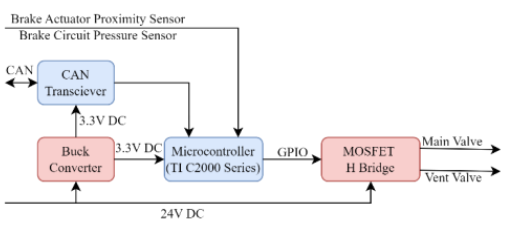
\includegraphics{texfiles/elec/eimg/Brakes_architecture}
        \caption{Brakes Controller NAP Connections}
        \label{fig:Brakes Controller NAP Connections}
    \end{figure}
 \begin{figure}
        \centering
        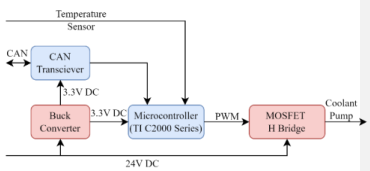
\includegraphics{texfiles/elec/eimg/Thermal_architecture}
        \caption{Thermal Controller NAP Connections}
        \label{fig:Thermal Controller NAP Connections}
    \end{figure}
 \begin{figure}
        \centering
        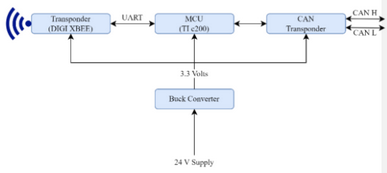
\includegraphics[width=\textwidth]{texfiles/elec/eimg/telem_architecture.png}
        \caption{Telemetry Unit Hardware Architecture}
        \label{fig:Telemetry Unit Hardware Architecture}
    \end{figure}

    \item Communication protocols used:
\begin{enumerate}
    \item Control Area Network (CAN): CAN employs collision-free communication through priority-based arbitration, error detection, and fault tolerance mechanisms, enabling real-time data exchange between electronic control units for efficient and reliable control of distributed systems. Taking all of this advantages into account, it was implemented to manage the inter-board  communication.

    \item WLAN: Used to transmit data between the Telemetry Unit and command PC.

    \item Serial Peripheral Interface (SPI): Synchronous, full-duplex communication protocol used for connecting peripheral devices.The master device generates the clock signal on SCLK while transmitting data to the slave device via MOSI, and the slave device responds with data on MISO. Communication occurs simultaneously in both directions, what allows high-speed data transfer between devices.

    \item Inter-Integrated Circuit (I2C): Synchronous, multi-master, multi-slave communication protocol used for connecting low-speed peripherals. Devices communicate by addressing one another with unique addresses. This way, a single master is able to control multiple slave devices on the same bus through packet-switched data exchanges. 
\end{enumerate}

\end{enumerate}

Both SPI and I2C were applied for the accelerometer readings in the breaking system.
% Merged detailed content from the first snippet

\subsection{State Machine of the Vehicle}
% Continue with the structured format from the second snippet, ensuring to merge relevant content from the first snippet into these sections.

We use different states in each component. Generally (and in the main control of the pod), we have the following structure:

\subsection{Code Architecture and Class Diagram}
% Insert content from the first snippet related to Code Architecture here.
\subsubsection{Brakes Controller}
The software follow a simple state: \\

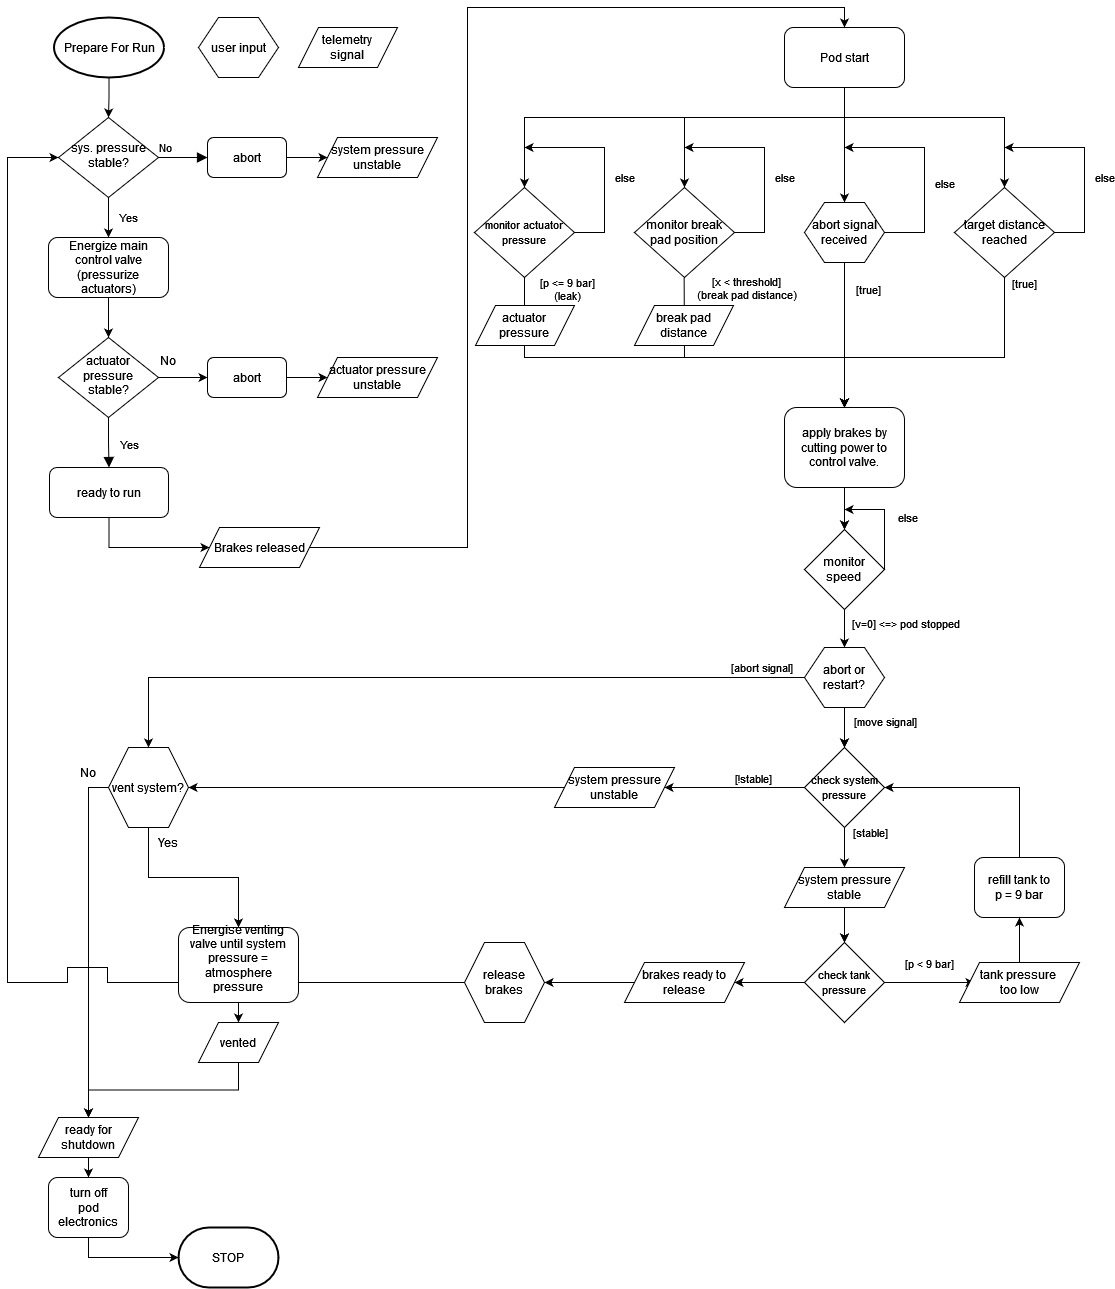
\includegraphics[width=\textwidth]{texfiles/elec/eimg/brakesoftware_ext}

\subsubsection{Thermal Controller}
Software goes along the following state diagram: \\
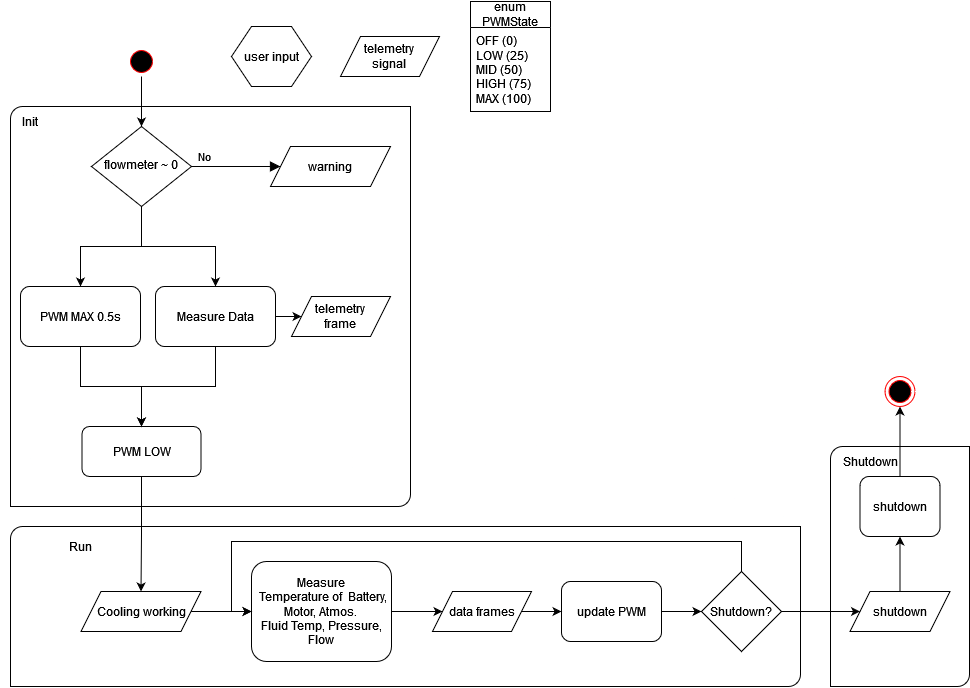
\includegraphics[width=\textwidth]{texfiles/elec/eimg/thermalsystemsflowchartsoftware}

The following hardware architecture is to be implemented:

\subsubsection{Telemetry Device}
The software adheres to this chart:
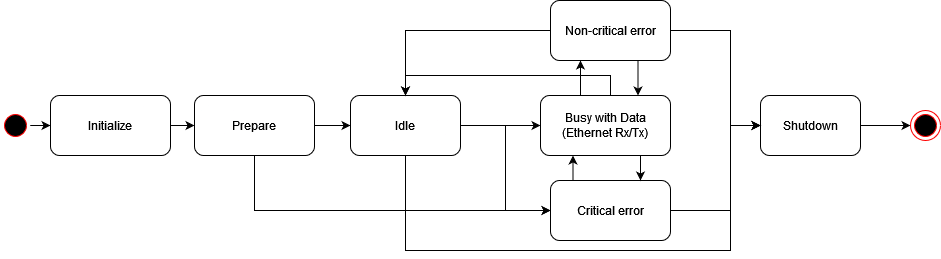
\includegraphics[width=\textwidth]{texfiles/elec/eimg/telemetrystate.png}

\subsection{Control Boards/Units in the Vehicle}
% Insert content from the first snippet related to Control Boards/Units in the Vehicle here.

\begin{enumerate}
    \item Brakes Controller
    \begin{enumerate}
        \item Requirements of the board.
        Parts List:
            \begin{table}[h]
                \centering
                \begin{tabular}{|c|c|c|c|c|c|c|}
                \hline
                \textbf{Amount} & \textbf{Name} & \textbf{Company (Serial Number)} & \textbf{Dimensions (mm x mm x mm)} & \textbf{Weight (kg)} & \textbf{Nominal Voltage} & \textbf{Expected max current} \\
                \hline
                38 & Additional Temperature Sensors (NTC, 10k Ohm) & Mouser & 1000 x 3 x 3 & $200 \times 10^{-6}$ & - & - \\
                \hline
                1 & Coolant Pump & Unknown & Unknown & Unknown & Unknown & Unknown \\
                \hline
                1 & MOSFET Bridge & Unknown & Unknown & Unknown & Unknown & Unknown \\
                \hline
                \end{tabular}
                \caption{Description of Components}
                \label{tab:components}
            \end{table}
        \item Hardware Rationale (HW design and concerns).

        \item Firmware Rationale (Internal State machine and design concerns).

        \item Testing and validation plan.


    \end{enumerate}

    \item Thermal Controller
        \begin{enumerate}
            \item Requirements of the board.

            \item Hardware Rationale (HW design and concerns).

            \item Firmware Rationale (Internal State machine and design concerns).

            \item Testing and validation plan.
        \end{enumerate}

\item Telemetry Controller
        \begin{enumerate}
            \item Requirements of the board.
            Parts Lists
                \begin{table}[H]
                    \centering
                    \begin{tabular}{|l|l|l|}
                    \hline
                    \textbf{Part} & \textbf{Manufacturer} & \textbf{Description} \\ \hline
                    Raspberry Pi Zero 2 W & Raspberry & Microcontroller for telemetry \\ \hline
                    Raspberry Pi 4 B & Raspberry & Computer for telemetry \\ \hline
                    MC3479 & Memsic & 3-Axis Accelerometer \\ \hline
                    RS485 CAN HAT & Waveshare & CAN adapter for RPI4B \\ \hline
                    \end{tabular}
                    \caption{Telemetry System Parts List}
                    \label{tab:my-table}
                \end{table}
            \item Hardware Rationale (HW design and concerns).
            
            \item Firmware Rationale (Internal State machine and design concerns).

            \item Testing and validation plan.
        \end{enumerate}
\end{enumerate}

\subsection{Communication and Navigation}
For communication and navigation, we use our telemetry system, that consists of a CAN bus, a CAN2WLAN transmitter and a VCU.

\begin{enumerate}
    \item Design requirements
The Telemetry Devices possesses the following properties and constraints

\begin{table}[htbp]
    \centering
    \begin{tabular}{|l|l|}
        \toprule
        \textbf{Constraint/Specification} & \textbf{Value} \\
        \midrule
        Operating Voltage & 24 V \\
        Mass & $<200$ g \\
        Budget & $<500$ € \\
        Range & 1.2 Km LOS \\
        Communication Frequency & 2.4GHz \\
        \bottomrule
    \end{tabular}
     \caption{Specification of the Telemetry Unit Constraints}
\label{tab:Telemetry Constraints}
\end{table}

To allow the correct transmission of information, the following CAN signals should be sent by the Telemetry unit to all the Slave devices:
\begin{table}[htbp]
    \centering
    \begin{tabular}{|l|l|}
        \textbf{Device} & \textbf{Command} \\
        \midrule
        Traction Controller & Target Speed or Torque \\
        Battery Pack & Emergency Disconnect \\
        Thermal Management System & Target Temperature \\
        Brakes Controller & Brake Engage Command \\
        \bottomrule
    \end{tabular}
 \caption{Devices and their commands}
\label{tab:Command devices.}
\end{table}

\begin{table}[htbp]
    \centering
    \begin{tabular}{|l|l|}
        \toprule
        \textbf{Device} & \textbf{Signal} \\
        \midrule
        All & Emergency / Error Messages \\
        Traction Controller & Speed, Phase Currents, Inverter Module \& Motor Temperature \\
        Battery Pack & Pack Voltage, Pack Current, Cell Temperatures, SoC \\
        Thermal Systems & Temperatures \\
        \bottomrule
    \end{tabular}
    \caption{CAN signals received by the devices}
\label{tab:CAN signals.}
\end{table}

All the above signals shall be transmitted to the command PC over Wireless communication.

    \item Network Diagrams:
The overall system can be described with the following chart:
\begin{figure}
    \centering
    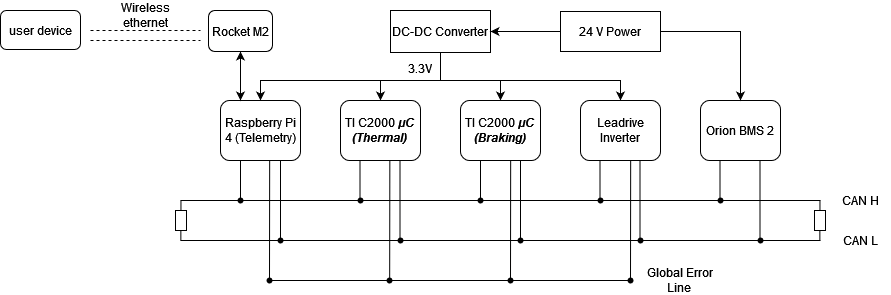
\includegraphics[width=\textwidth]{texfiles/elec/eimg/telemetrysystems.png}
    \caption{Overall Structure of the Telemetry Sytem}
    \label{fig:enter-label}
\end{figure}
%I dont think we have
    \item Sub-networks Diagrams (Track, Vehicle and Spectators)

    \item Graphical User Interface (GUI)
\end{enumerate}


% Shouldn´t be added imo
\subsection{Integration with other systems}
The friction brakes, the cooling pump and the motor are controlled through our system.

% Insert content from the first snippet related to GUI here.

% Continue merging additional sections and sub-sections from the first snippet into the structured format of the second snippet as needed.

